\begin{frame}
\begin{figure}

\vspace{-.7cm}	
\hspace{-2cm}		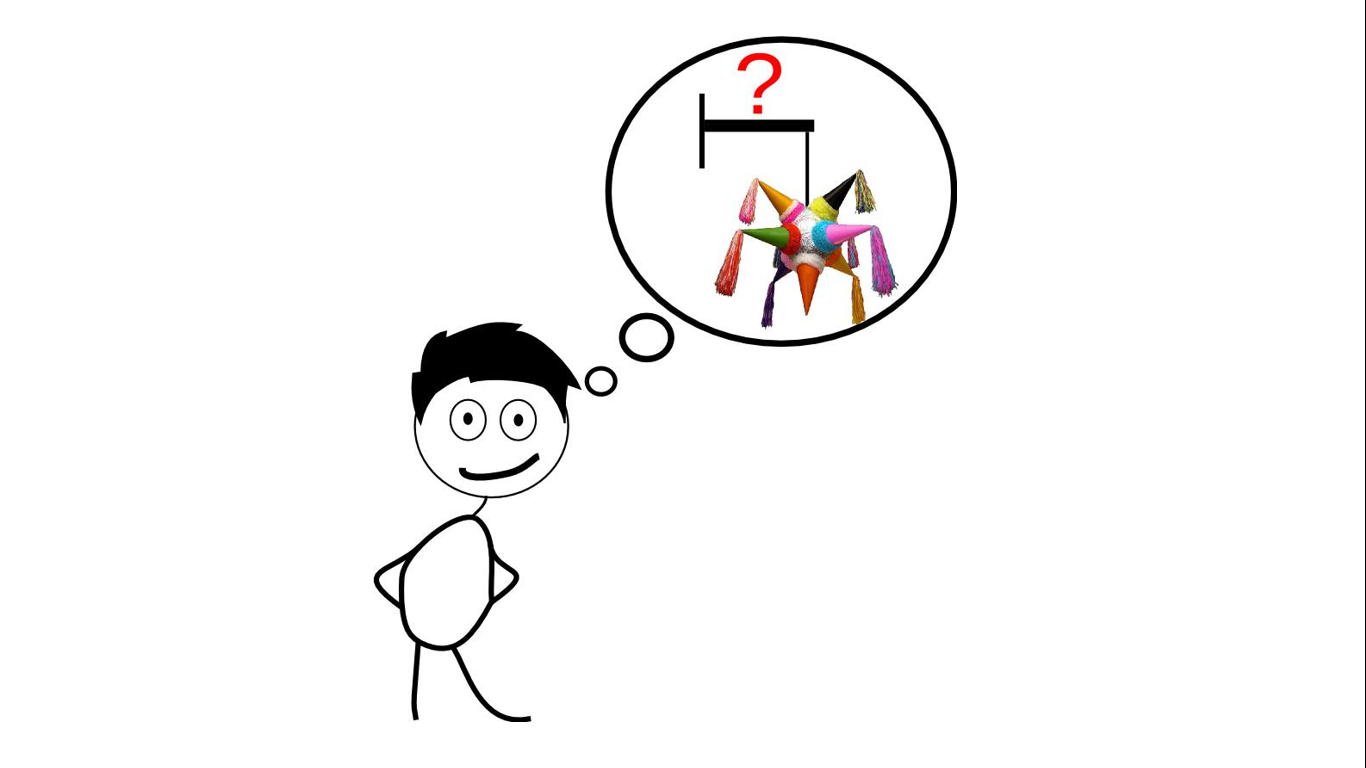
\includegraphics[width=1.2\linewidth]{Pictures/animations/animation_1_1.png}
		\end{figure}

\end{frame}

\begin{frame}
\begin{figure}

\vspace{-.7cm}	
\hspace{-2cm}		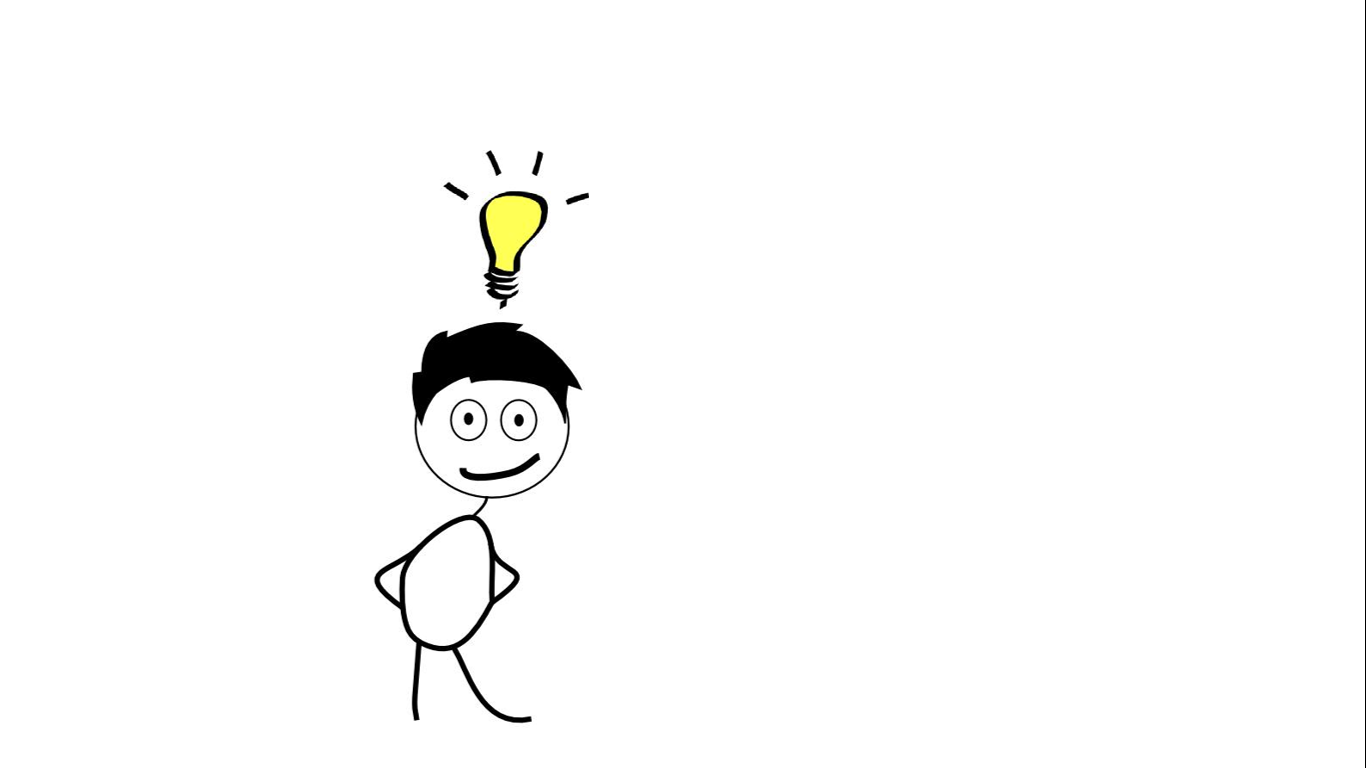
\includegraphics[width=1.2\linewidth]{Pictures/animations/animation_2_2.png}
		\end{figure}

\end{frame}

\begin{frame}
\begin{figure}

\vspace{-.7cm}	
\hspace{-2cm}		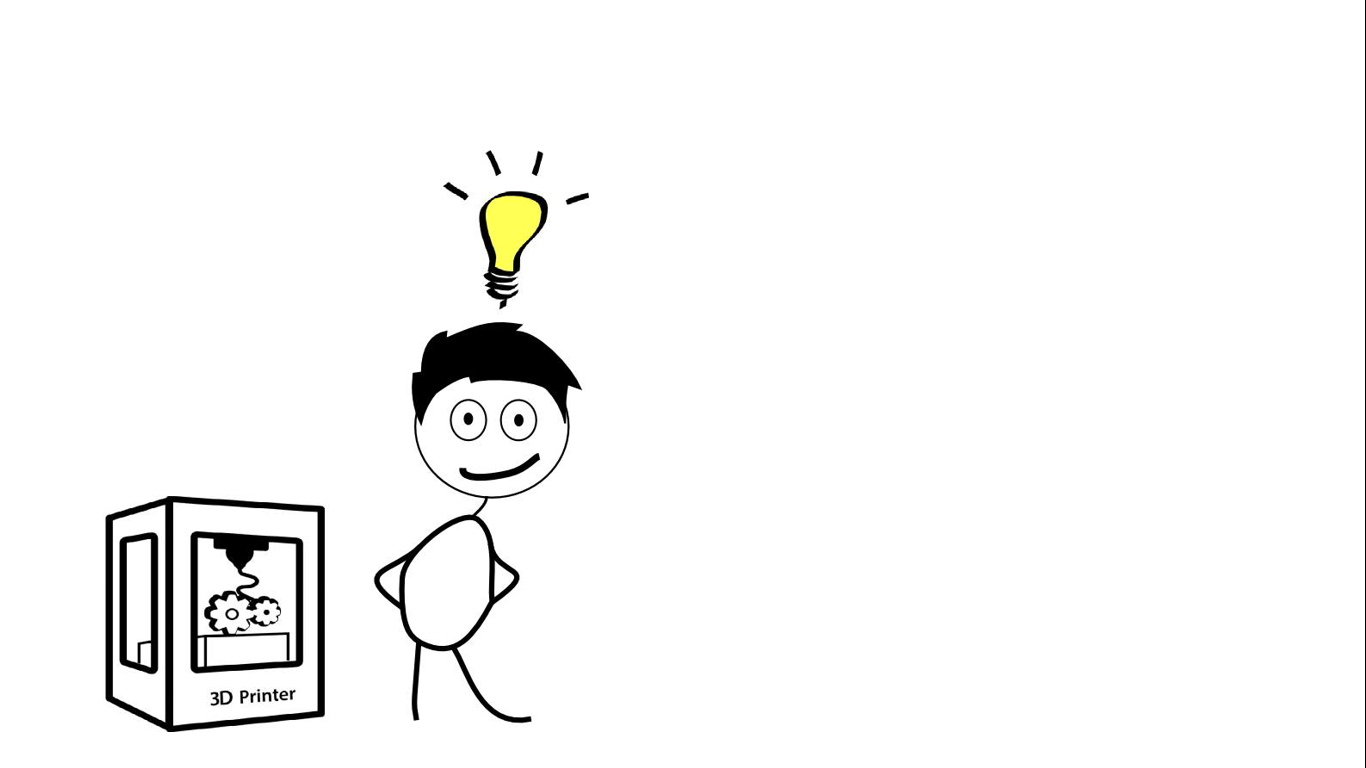
\includegraphics[width=1.2\linewidth]{Pictures/animations/animation_3.png}
		\end{figure}

\end{frame}

\begin{frame}
\begin{figure}

\vspace{-.7cm}	
\hspace{-2cm}		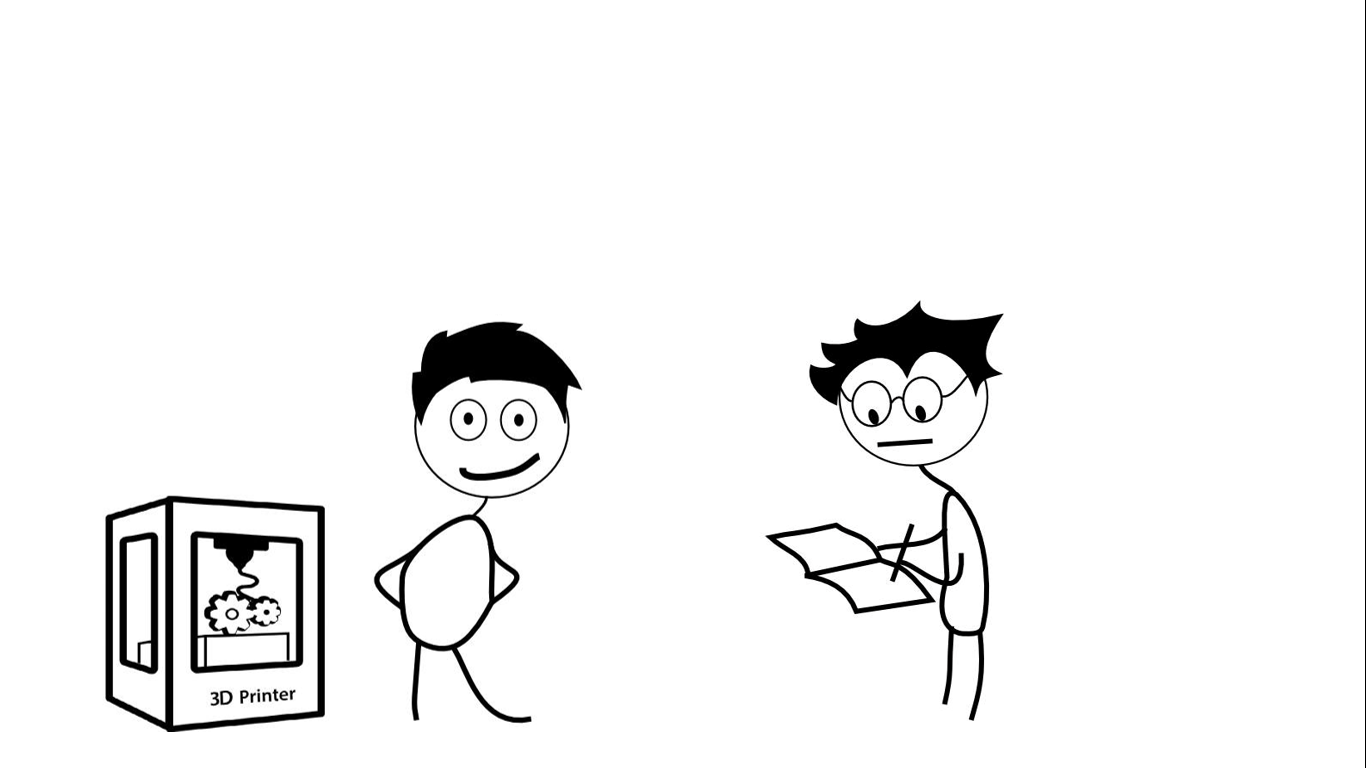
\includegraphics[width=1.2\linewidth]{Pictures/animations/animation_4.png}
		\end{figure}

\end{frame}

\begin{frame}
\begin{figure}

\vspace{-.7cm}	
\hspace{-2cm}		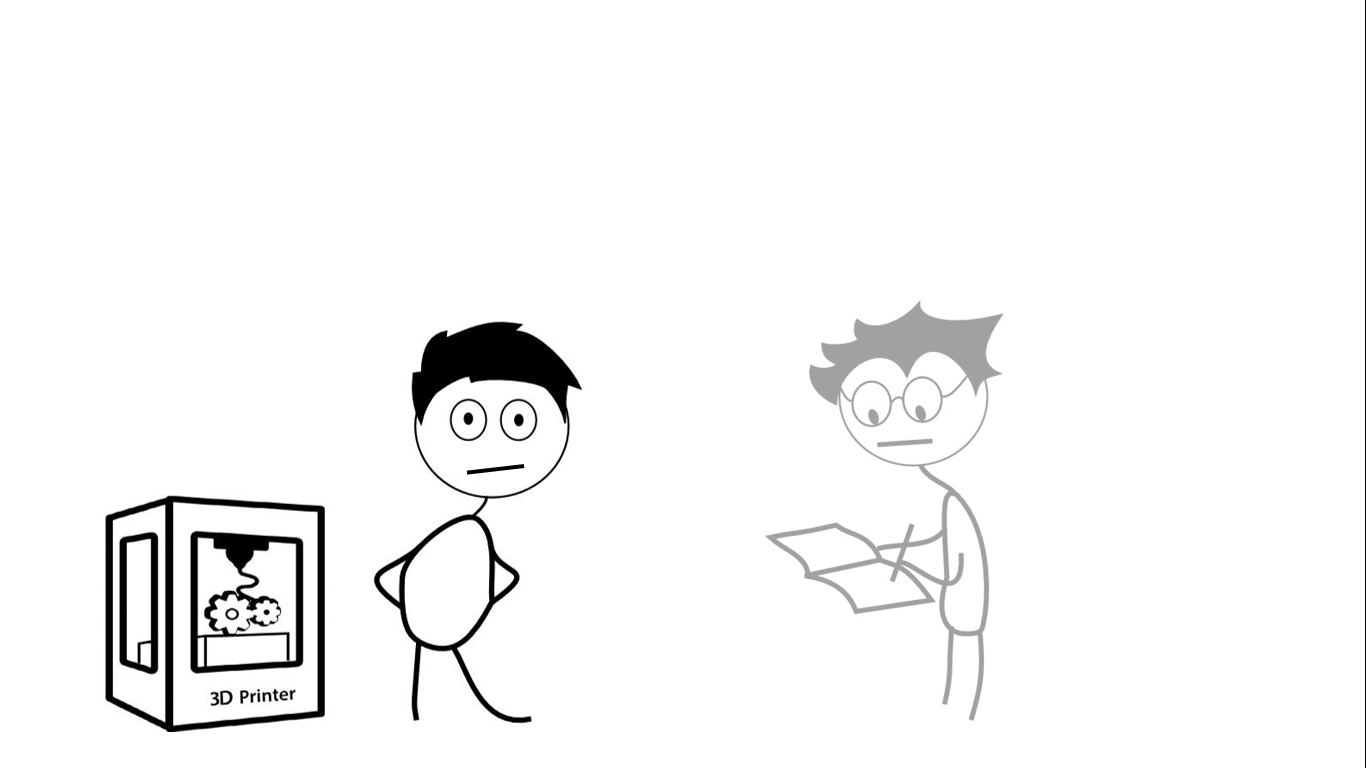
\includegraphics[width=1.2\linewidth]{Pictures/animations/animation_5.png}
		\end{figure}

\end{frame}

\begin{frame}
\begin{figure}

\vspace{-.7cm}	
\hspace{-2cm}		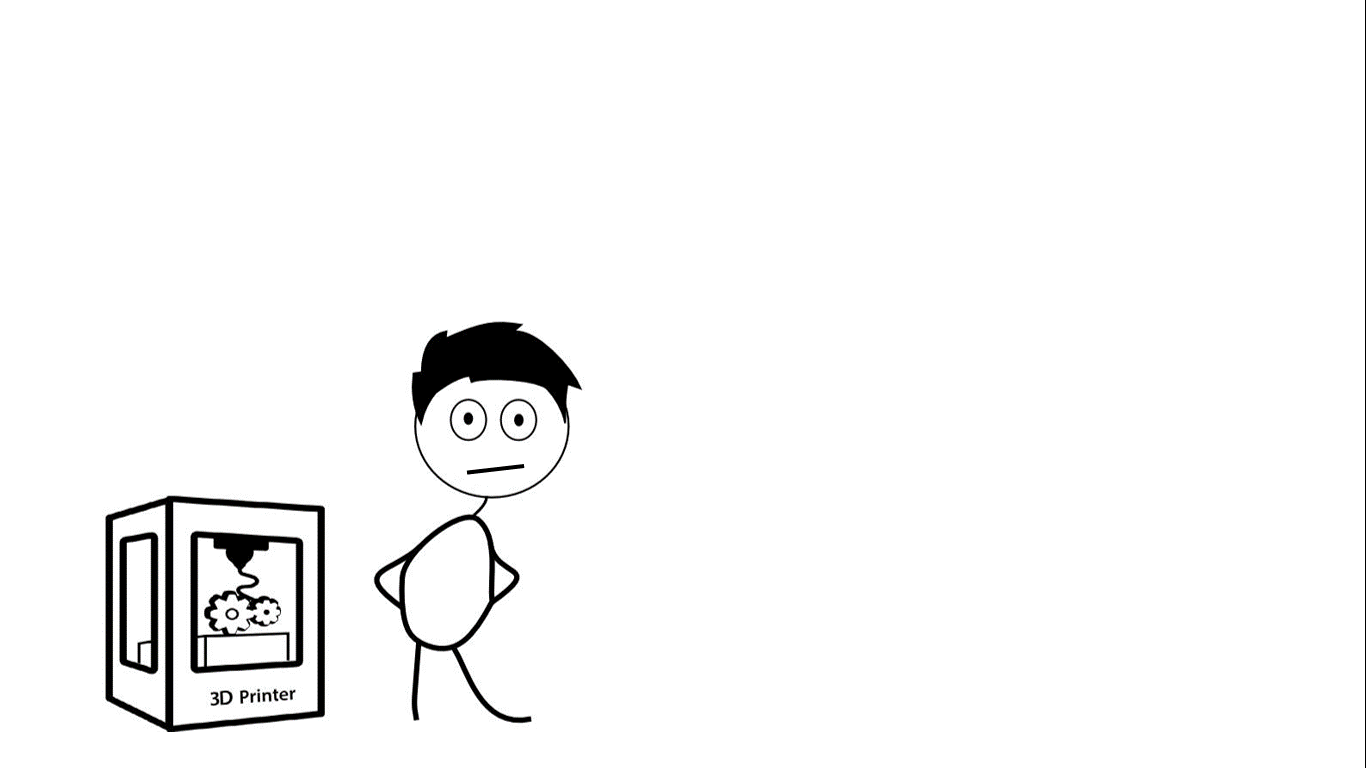
\includegraphics[width=1.2\linewidth]{Pictures/animations/animation_6.png}
		\end{figure}

\end{frame}

\begin{frame}
\begin{figure}

\vspace{-.7cm}	
\hspace{-2cm}		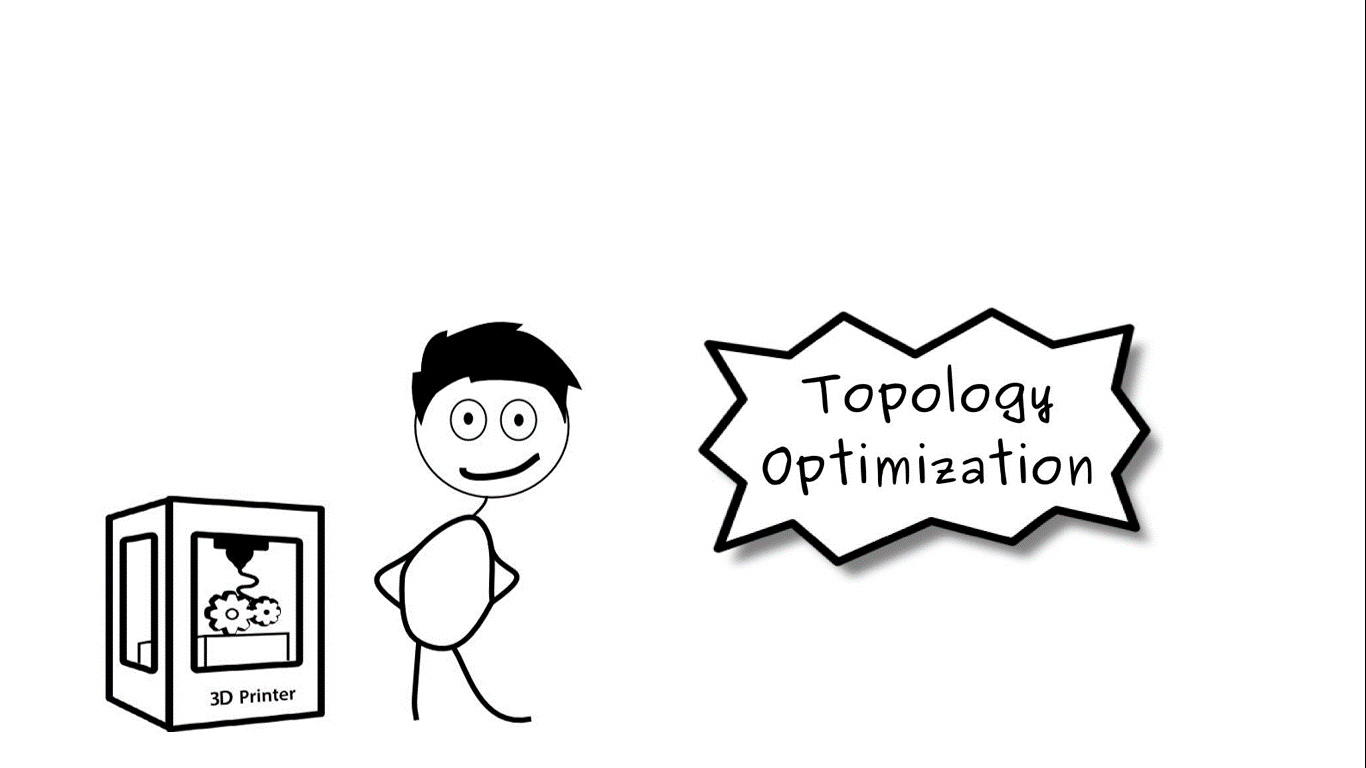
\includegraphics[width=1.2\linewidth]{Pictures/animations/animation_7.png}
		\end{figure}

\end{frame}

\begin{frame}
\begin{figure}

\vspace{-.7cm}	
\hspace{-2cm}		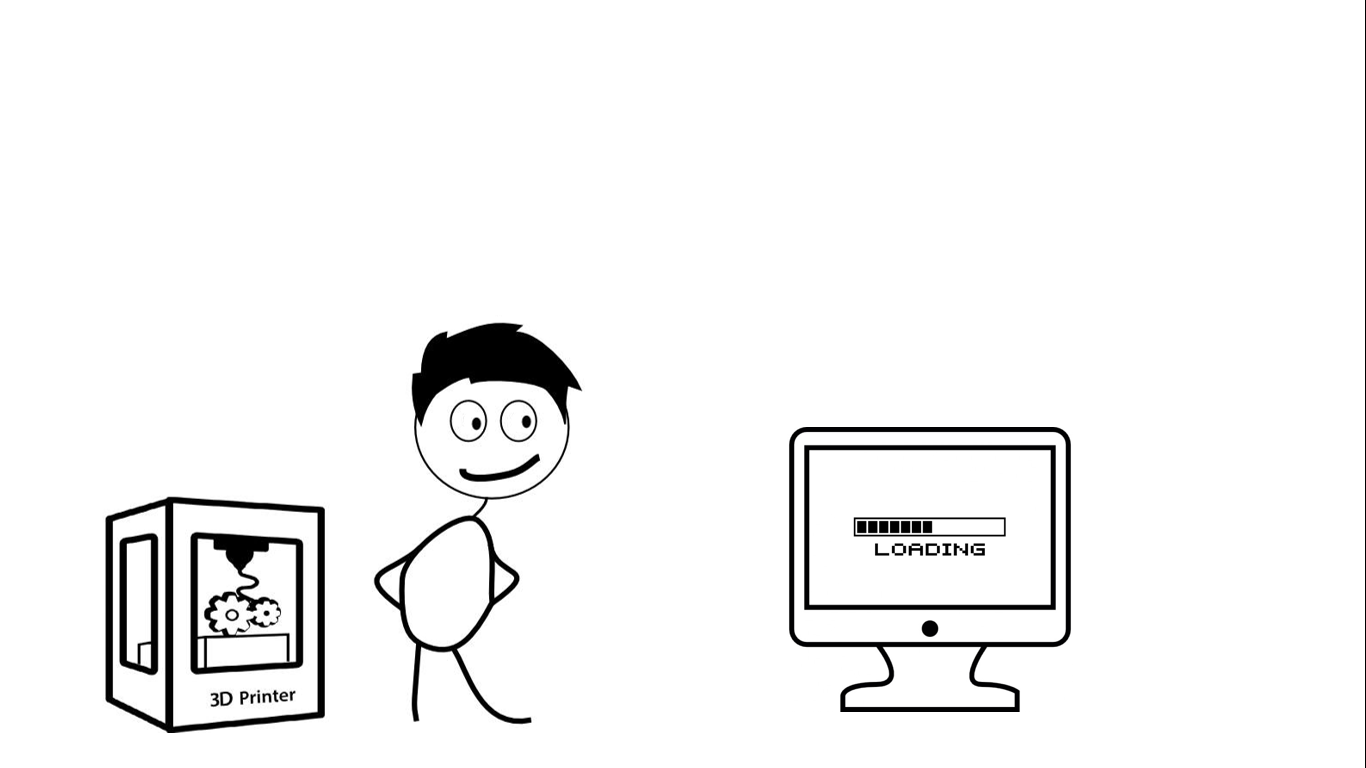
\includegraphics[width=1.2\linewidth]{Pictures/animations/animation_8.png}
		\end{figure}

\end{frame}

\begin{frame}
\begin{figure}

\vspace{-.7cm}	
\hspace{-2cm}		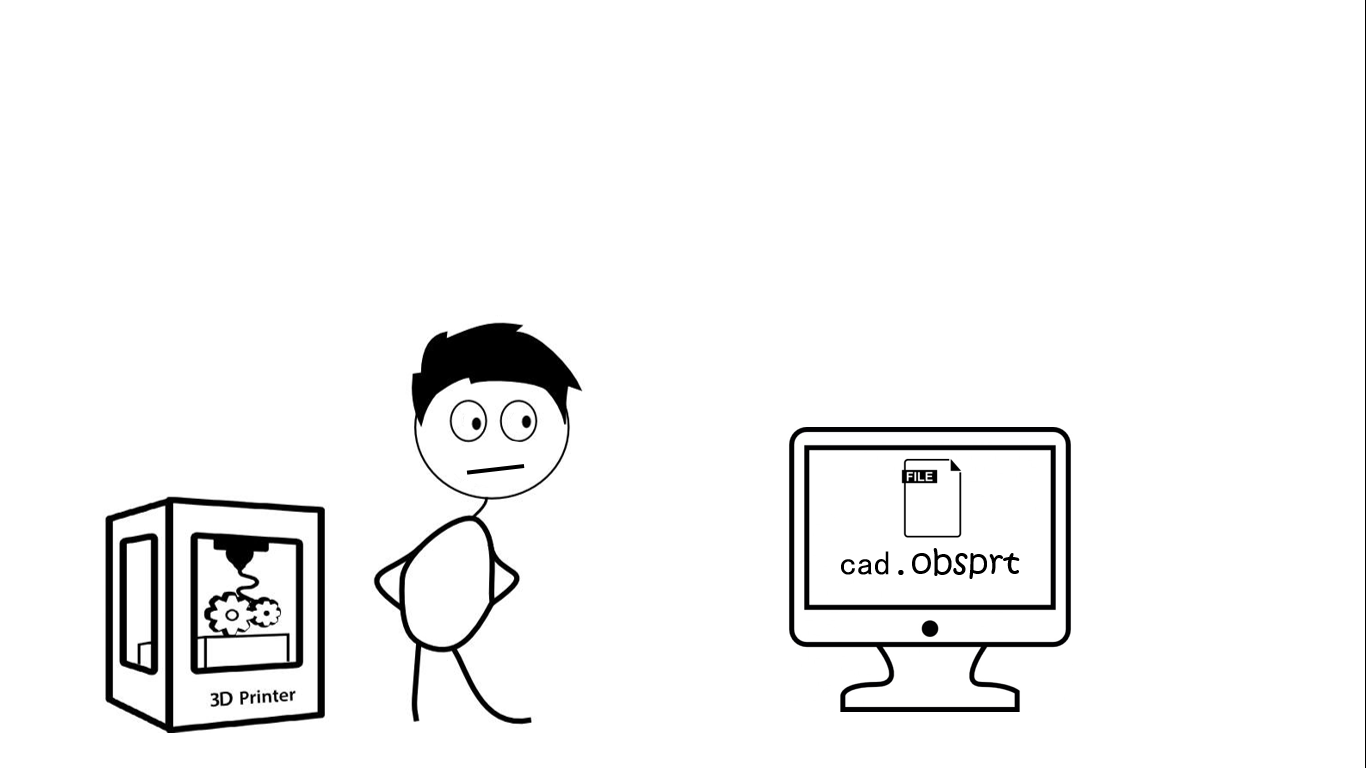
\includegraphics[width=1.2\linewidth]{Pictures/animations/animation_9.png}
		\end{figure}

\end{frame}

\begin{frame}{Design Issues}
	
	
\includegraphics[width=0.175\textwidth, center]{Pictures/animations/animation_designer_sad}
	
	\begin{multicols}{2}
		%\underline{Problem:}
		\setbeamercolor{block}{bg=white,fg=cyan}
		\begin{block}{Status-quo:}{
				\begin{itemize}		
					\item Engineering-design processes are a pendulum
					\item Topology-Optimization algorithms are a one-way street
				\end{itemize}~\\
			}
			%\begin{variableblock}{Focus:}{bg=cyan,fg=white}	
		\end{block}
		\pause
		\columnbreak
		
		\begin{block}{Objectives:}{
				\begin{itemize}		
					\item[$\Rightarrow$] One-click optimization
				\end{itemize}
				\begin{itemize}		
					\item[$\Rightarrow$] Full-circle process
				\end{itemize}
			}
		\end{block}
		
	\end{multicols}
	
\end{frame}	

\begin{frame}{Introducing..}
	\begin{figure}
		\centering
		
\includegraphics[scale=0.7]{Pictures/FirstHalf/Intro_slide.pdf}
	\end{figure}
	\begin{figure}
		\centering
		
\includegraphics[scale=0.35]{Pictures/FirstHalf/sccs_os2.pdf}
	\end{figure}
\end{frame}

% FEATURES
\begin{frame}{Features}
	\begin{block}{Effective and Easy}{
			\begin{itemize}
				\item Reconstructs 3D geometry from Top-opt results
				\item Provides production-ready output
				\item Works like a black-box
			\end{itemize}
		}
	\end{block}
	\pause
	\begin{block}{Customizable}{
			You can specify:
			\begin{itemize}
				\item detailed geometry and boundary conditions
				\item optimization accuracy
				\item surface quality and smoothness
			\end{itemize}
		}
	\end{block}
	\pause
	\begin{block}{100\% open source!}{
			%\begin{itemize}		
			%\end{itemize}~\\
		}
	\end{block}
\end{frame}

\begin{frame}{Time to help Dave!}
	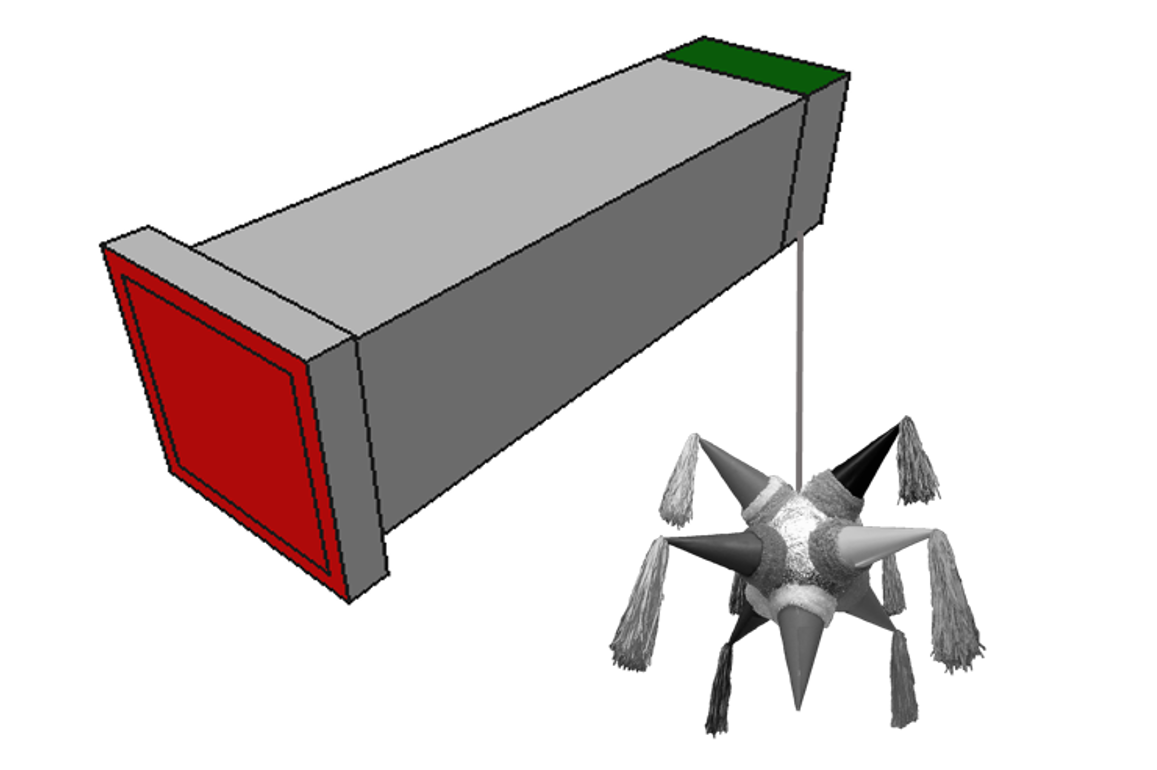
\includegraphics[width=0.75\textwidth, center]{Pictures/FirstHalf/pinata}
\end{frame}

\begin{frame}{Time to help Dave!}
	
\includegraphics[width=0.3\textwidth, center]{Pictures/FirstHalf/alarm}
\end{frame}